\documentclass{IEEEtran}

\usepackage[utf8]{inputenc}
\usepackage{lipsum}
\usepackage{subfig}
\usepackage{graphicx}

\title{Lorem Ipsum}

\author{Me and Me}
\begin{document}
\maketitle

\begin{abstract}
\lipsum[1-2]
\end{abstract}

\section{Introdução}
\lipsum[3-4]
\section{Estado da Arte}
\lipsum[4-5]
\section{Métodos}
\lipsum[6-8]

Flowers in my garden can be depicted in Figure~\ref{fig:one}.
\begin{figure*}[!t]
\subfloat[Flor 1.]{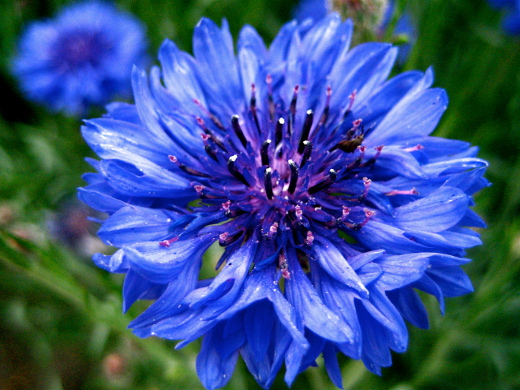
\includegraphics[width=0.2\textwidth]{imgs/1.jpg}}
\subfloat[Flor 2.]{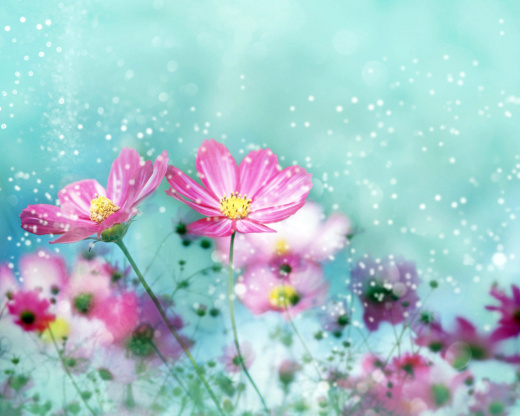
\includegraphics[width=0.2\textwidth]{imgs/2.jpg}}
\subfloat[Flor 3.]{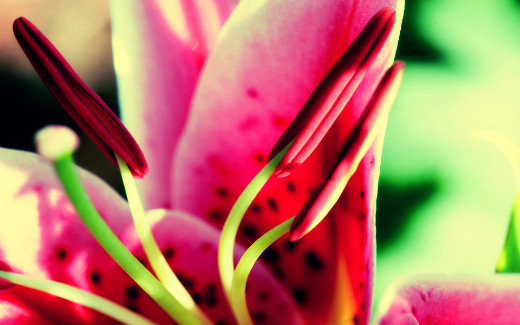
\includegraphics[width=0.2\textwidth]{imgs/3.jpg}}
\subfloat[Flor 4.]{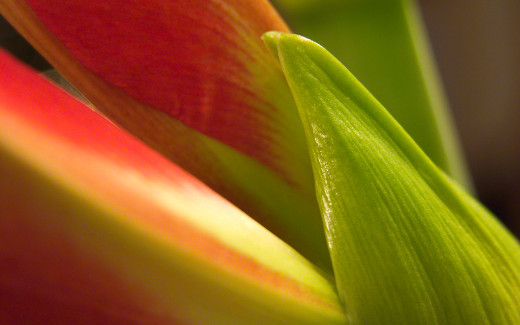
\includegraphics[width=0.2\textwidth]{imgs/4.jpg}}
\subfloat[Flor 5.]{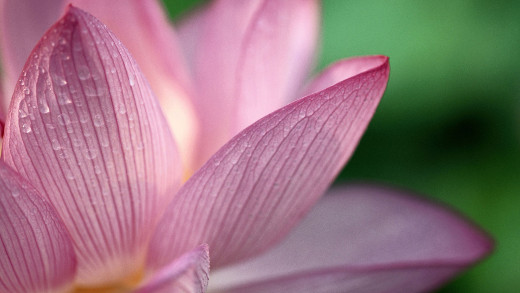
\includegraphics[width=0.2\textwidth]{imgs/5.jpg}}

\subfloat[Flor 6.]{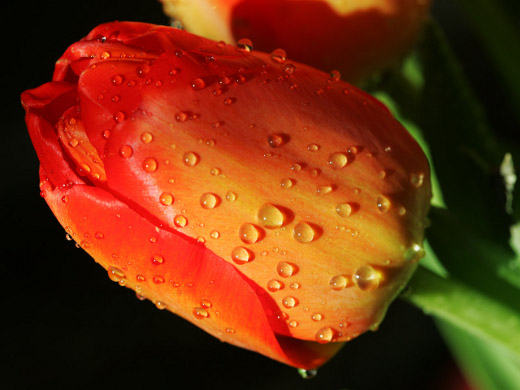
\includegraphics[width=0.2\textwidth]{imgs/6.jpg}}
\subfloat[Flor 7.]{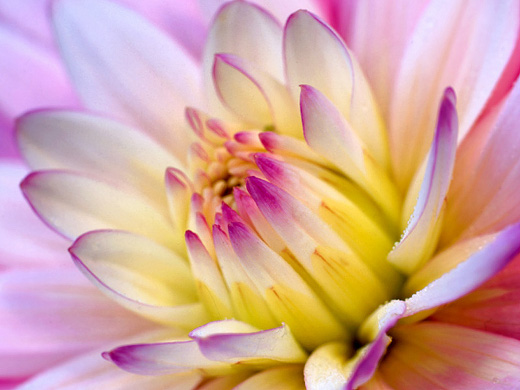
\includegraphics[width=0.2\textwidth]{imgs/7.jpg}}
\subfloat[Flor 8.]{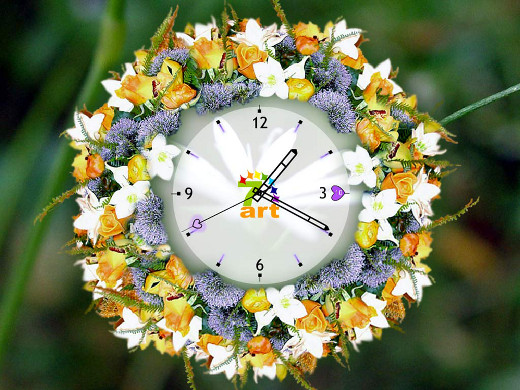
\includegraphics[width=0.2\textwidth]{imgs/8.jpg}}
\subfloat[Flor 9.]{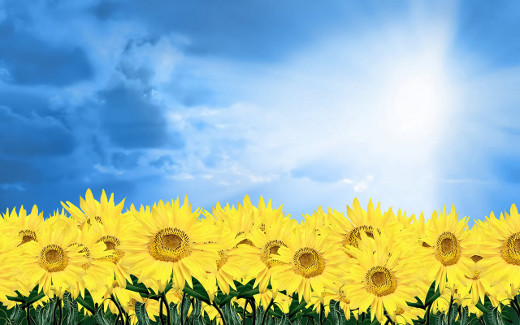
\includegraphics[width=0.2\textwidth]{imgs/9.jpg}}
\subfloat[Flor 10.]{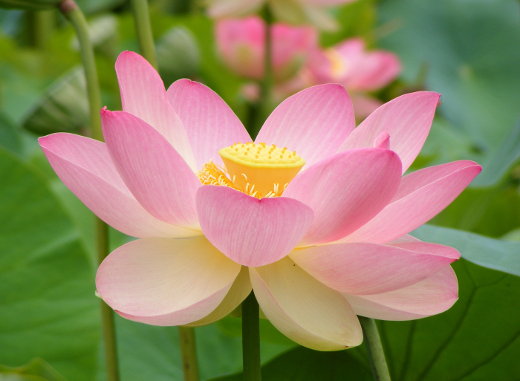
\includegraphics[width=0.2\textwidth]{imgs/10.jpg}}
\caption{Flowers of different kinds and colors.}
\label{fig:one}
\end{figure*}

\lipsum[9-10]

\lipsum[11-20]

\cite{TPJ}
\cite{bishop2012light}


\section{Discussão}
\lipsum[21-23]
\section{Conclusão}
\lipsum[24-25]

\bibliographystyle{IEEEtran}
\bibliography{refs}


\end{document}
